\documentclass{article}
\usepackage[textwidth=14cm]{geometry}
\usepackage[title]{appendix}
\usepackage[utf8]{inputenc}
\usepackage{amsmath}
\usepackage{physics}
\usepackage{graphicx}
\usepackage{mathtools}
\usepackage{subcaption}
\usepackage{hyperref}
\usepackage{fancyhdr}
\usepackage{float}
\usepackage{abstract}
\usepackage{lipsum}
\usepackage[english]{babel}
\usepackage[export]{adjustbox}[2011/08/13]
\usepackage{biblatex}
\addbibresource{Reference.bib}
\usepackage[flushleft]{threeparttable}
\usepackage{array,booktabs,makecell}
\usepackage{multirow}
\usepackage{floatrow}


\usepackage[table,xcdraw]{xcolor}
\renewcommand{\abstractname}{}
\renewcommand{\absnamepos}{empty} 
\hypersetup{
    colorlinks=true,
    linkcolor=blue,
    filecolor=magenta,      
    urlcolor=cyan,
}


\newcommand{\fsl}[1]{\ensuremath{\mathrlap{\!\not{\phantom{#1}}}#1}}% fsl{<symbol>}
\usepackage{tikz} 
\usetikzlibrary{shapes,arrows,positioning,automata,backgrounds,calc,er,patterns}
\usepackage{tikz-feynman,contour}
\tikzfeynmanset{compat=1.0.0}
\begin{document}
\title{FYS5555 Project 1}
\date{}
\begin{titlepage}
\centering
{\LARGE\bfseries FYS5555 Project 3}

\vspace{1cm}

{\Large Searching for two direct sleptons in a proton-proton collison using supervised machine learning}

\vspace{1.5cm}

{\large William Hirst}

\vspace{1cm}

{\bfseries Spring 2022}

\vspace{2cm}

\begin{figure}[H]
    \centering
    \includegraphics[width=0.8\linewidth]{Figures/Illustrations/signal.png}
    \label{fig:signal}
\end{figure}

\vfill

{\itshape University of Oslo}
\end{titlepage}
\newpage
\pagestyle{fancy}
\fancyfoot{}
\fancyfoot[R]{\thepage}

\begin{center}
\centering
\textit{
In this rapport I will be studying the higgs decay in a proton proton collision.  
}
\end{center}
\section{Introduction}
Some of the theory and ideas in this rapport are based on and will hope to build on the work by the ATLAS Collaboration  in 2013 \cite{ATLAS2012} and 2020 \cite{Aad_2020}. 
\\
\section{Theory}
In this section I will discuss the necessary theory for both the physical analysis (supersymmetry, statistical tools ect.) as well as the tools need for the ML analysis. Note that the sections on ML methods is taken from my previous work in the articles \cite{FYSSTK} and \cite{HIGGS}.
\subsection{Basic search strategy}
In most attempts to search for beyond the standard model (BSM) physics the basic idea is to define a new model of interest and compare Monte Carlo data (MC) with with real data in designated regions we call signal regions (SR). To define these SR we use MC-data. As will be made clearer in later section, we want to define signal regions as a region in feature space with the most amount of predicted MC-data of the BSM physics of choice (signal) and the least amount of SM MC-data (background). Defining these regions can sometimes be done through classical rectangle cuts in certain features. Using machine learning in such searches allows us to define more sophisticated cuts based on trends in the features space that might be not visible to the human eye.
\subsection{Super symmetry}
A supersymmetric theory has for many years been an interesting candidate for a new physics beyond the standard model. Supersymmetry (SUSY) aims to alter the standard model such that mass and force is treated equally. Supersymmetry suggests that each SM particle has an additional superpartner(SP) which we call a sparticle. The sparticles all differs with half a spin from the original SM particle. Because SUSY is a broken symmetry, sparticles are expected to be much higher than the corresponding SM masses, often in the range of 100-1000GeV. The difference in spin means that the SP of a fermion is a boson and the SP of a boson is a fermion. SUSY is a candidate to fix many problems in physics, some of which are; the hierarchy problem, fixing the mass of the higgs and possibly the mystery of dark matter.
\\
In this analysis I have chosen to search for supersymmetry through the signal of two direct sleptons decaying to a lepton and a neutralino. The process closely resembles the Drell-Yan production, but with additional neutralinos. The diagram is shown in figure \ref{fig:signal_f}. In the rapport only the sleptons $\tilde{e}$ and $\tilde{\mu}$ (SP of ${e}$ and ${\mu}$) will be considered.
\\
In the paper from F. del Aguila and Ll. Ametller \cite{DELAGUILA1991326}, they argue that the slepton should be detectable at the LHC with masses up to 250GeV. In addition SUSY predicts that all SP will have masses between 100GeV-1Tev. Therefore the range of mass of the slepton in this analysis will be in the range of 100-250GeV.
\begin{figure}[H]
    \centering
    \begin{tikzpicture}
    \begin{feynman}
        \vertex at (-1.75, 1.1) (i1) {\(P\)};
        \vertex at (-1.5, 1.) (i2);
        \vertex at (-1.525, 0.9) (i3) ;
        \vertex at (0.18, 1.1)  (a1);
        \vertex at (0.5, 1.) [blob] (a2) {\contour{white}};
        \vertex at (0.18, 0.9) (a3);
        
        \vertex at (-1.75, -1.1) (i4) {\(P\)};
        \vertex at (-1.5, -1.) (i5);
        \vertex at (-1.525, -0.9) (i6) ;
        \vertex at (0.18, -1.1)  (a4);
        \vertex at (0.5, -1.) [blob] (a5) {\contour{white}};
        \vertex at (0.18, -0.9) (a6);
        
        \vertex at (1.25, 0.0) (c);
        \vertex at (3., 0.0) (d);
        \vertex at (1,-0.5) (b);
        
        \vertex at (3.5, 1.) (f1) ;
        \vertex at (3.5,-1.) (f2);
        \vertex at (5.5, 1.5) (f3) {\(l^-\)};
        \vertex at (5.5, 0.5) (f4) {\(\tilde{\chi}_1^0\)};
        \vertex at (5.5, -0.5) (f5) {\(\tilde{\chi}_1^0\)};
        \vertex at (5.5, -1.5) (f6) {\(l^+\)};
        
    \diagram*{
        (i1) -- [lepton] (a1) ,
        (i2) -- [fermion] (a2) [blob],
        (i3) -- [lepton] (a3), 
        (a2) -- [fermion] (c) -- [boson] (d),
        (i4) -- [lepton] (a4) ,
        (i5) -- [fermion] (a5) [blob],
        (i6) -- [lepton] (a6), 
        (a5) -- [anti fermion] (c) -- [boson, edge label = {$Z,\gamma$}] (d),
        (d) -- [fermion, edge label =\(\tilde{l}^-\) ] (f1),
        (d) -- [fermion, edge label =\(\tilde{l}^+\) ] (f2),
        (f1) -- [fermion] (f3),
        (f1) -- [ghost] (f4),
        (f2) -- [anti fermion] (f6),
        (f2) -- [ghost] (f5),
        ;
    };
    \end{feynman}
    \end{tikzpicture}
    \caption{The Feynman diagram for the direct slepton signal channel.}
    \label{fig:signal_f}
\end{figure}
Why search for neutralinos? Version of SUSY suggest an introduction of a new quantum number, R parity. The new quantum number suggests that the lightest neutralions do not decay into SM particles. Given it is neutral, this makes it a prime candidate for DM.
\subsection{Standard model background}
In the analysis of direct slepton signal there are several background channels of interest. In this rapport only a handful of the aforementioned channels were included in the rapport given the limits of computational power and time. The channels were included based on there relevance. 
\subsubsection{Dibson ($WW,WZ,ZZ$)}
Based on the results in the ATLAS paiper, \cite{Aad_2020} the diboson channels seems to be the largest source of background events. This is partly due to the variation of diagrams, but most importantly the resemblance to the signal diagram. Three diboson channels are included in the analysis; $WW$, $WZ$ and $ZZ$.
\\
In figure \ref{fig:WW} I have drawn the Feynman diagram of the WW channel. The figures shows two quark-annihilation forming a neutral boson, which decays into a pair of W-bosons. The W-boson later decay into a pair of charged and neutral leptons. 
\begin{figure}[H]
    \centering
    \begin{tikzpicture}
    \begin{feynman}
        \vertex at (-1.75, 1.1) (i1) {\(P\)};
        \vertex at (-1.5, 1.) (i2);
        \vertex at (-1.525, 0.9) (i3) ;
        \vertex at (0.18, 1.1)  (a1);
        \vertex at (0.5, 1.) [blob] (a2) {\contour{white}};
        \vertex at (0.18, 0.9) (a3);
        
        \vertex at (-1.75, -1.1) (i4) {\(P\)};
        \vertex at (-1.5, -1.) (i5);
        \vertex at (-1.525, -0.9) (i6) ;
        \vertex at (0.18, -1.1)  (a4);
        \vertex at (0.5, -1.) [blob] (a5) {\contour{white}};
        \vertex at (0.18, -0.9) (a6);
        
        \vertex at (1.25, 0.0) (c);
        \vertex at (3., 0.0) (d);
        \vertex at (1,-0.5) (b);
        
        \vertex at (3.5, 1.) (f1) ;
        \vertex at (3.5,-1.) (f2);
        \vertex at (5.5, 1.5) (f3) {\(l^-\)};
        \vertex at (5.5, 0.5) (f4) {\(\bar{\nu}\)};
        \vertex at (5.5, -0.5) (f5) {\(\nu\)};
        \vertex at (5.5, -1.5) (f6) {\(l^+\)};
        
    \diagram*{
        (i1) -- [lepton] (a1) ,
        (i2) -- [fermion] (a2) [blob],
        (i3) -- [lepton] (a3), 
        (a2) -- [fermion] (c) -- [boson] (d),
        (i4) -- [lepton] (a4) ,
        (i5) -- [fermion] (a5) [blob],
        (i6) -- [lepton] (a6), 
        (a5) -- [anti fermion] (c) -- [boson, edge label = {$Z,\gamma$}] (d),
        (d) -- [boson, edge label =\(W^-\) ] (f1),
        (d) -- [boson, edge label =\(W^+\) ] (f2),
        (f1) -- [fermion] (f3),
        (f1) -- [lepton] (f4),
        (f2) -- [anti fermion] (f6),
        (f2) -- [lepton] (f5),
        ;
    };
    \end{feynman}
    \end{tikzpicture}
    \caption{The Feynman diagram for the background diboson channel $WW$.}
    \label{fig:WW}
\end{figure}
In figure \ref{fig:WZ} I have drawn the Feynman diagram of WZ. The figure shows a up quark annihilating coupled to a W-boson and a down quark, and a anti-down quark coupled to a the aforementioned down quark and a Z-boson. The W-boson decays into a charged and neutral lepton pair and the Z can decay into a pair quarks or leptons. 
\begin{figure}[H]
    \centering
    \begin{tikzpicture}
    \begin{feynman}
        \vertex at (-1.75, 1.1) (i1) {\(P\)};
        \vertex at (-1.5, 1.) (i2);
        \vertex at (-1.525, 0.9) (i3) ;
        \vertex at (0.18, 1.1)  (a1);
        \vertex at (0.5, 1.) [blob] (a2) {\contour{white}};
        \vertex at (0.18, 0.9) (a3);
        
        \vertex at (-1.75, -1.1) (i4) {\(P\)};
        \vertex at (-1.5, -1.) (i5);
        \vertex at (-1.525, -0.9) (i6) ;
        \vertex at (0.18, -1.1)  (a4);
        \vertex at (0.5, -1.) [blob] (a5) {\contour{white}};
        \vertex at (0.18, -0.9) (a6);
        
        \vertex at (2.0, 1.) (c1);
        \vertex at (2.0, -1.) (c2);
        \vertex at (4.0, 1.) (d1);
        \vertex at (4.0, -1.) (d2);
        \vertex at (1,-0.5) (b);
        
        \vertex at (5.5, 1.5) (f3) {\(l^-\)};
        \vertex at (5.5, 0.5) (f4) {\(\bar{\nu}\)};
        \vertex at (5.5, -0.5) (f5) {\(l^-\)};
        \vertex at (5.5, -1.5) (f6) {\(l^+\)};
        
    \diagram*{
        (i1) -- [lepton] (a1) ,
        (i2) -- [fermion] (a2) [blob],
        (i3) -- [lepton] (a3), 
        (a2) -- [fermion, edge label = {$u$}] (c1) -- [boson, edge label = {$W^+$}] (d1),
        (i4) -- [lepton] (a4) ,
        (i5) -- [fermion] (a5) [blob],
        (i6) -- [lepton] (a6), 
        (c1) -- [fermion] (c2),
        (a5) -- [anti fermion,, edge label = {$\bar{d}$}] (c2) -- [boson, edge label = {$Z$}] (d2),
        (d1) -- [fermion] (f3),
        (d1) -- [lepton] (f4),
        (d2) -- [anti fermion] (f6),
        (d2) -- [fermion] (f5),
        ;
    };
    \end{feynman}
    \end{tikzpicture}
    \caption{Feynman diagram for the background diboson channel WZ.}
    \label{fig:WZ}
\end{figure}
In figure \ref{fig:ZZ} I have drawn the Feyman diagram of the ZZ-channel. The figure shows a diagram resembling that of the WZ-channel but with two Z-bosons. In this case the most relevant process for this analysis is the on where one of the Z-bosons decays into a pair of charged leptons and the other decays into a pair of neutral leptons. 
\begin{figure}[H]
    \centering
    \begin{tikzpicture}
    \begin{feynman}
        \vertex at (-1.75, 1.1) (i1) {\(P\)};
        \vertex at (-1.5, 1.) (i2);
        \vertex at (-1.525, 0.9) (i3) ;
        \vertex at (0.18, 1.1)  (a1);
        \vertex at (0.5, 1.) [blob] (a2) {\contour{white}};
        \vertex at (0.18, 0.9) (a3);
        
        \vertex at (-1.75, -1.1) (i4) {\(P\)};
        \vertex at (-1.5, -1.) (i5);
        \vertex at (-1.525, -0.9) (i6) ;
        \vertex at (0.18, -1.1)  (a4);
        \vertex at (0.5, -1.) [blob] (a5) {\contour{white}};
        \vertex at (0.18, -0.9) (a6);
        
        \vertex at (2.0, 1.) (c1);
        \vertex at (2.0, -1.) (c2);
        \vertex at (4.0, 1.) (d1);
        \vertex at (4.0, -1.) (d2);
        \vertex at (1,-0.5) (b);
        
        \vertex at (5.5, 1.5) (f3) {\(l^-\)};
        \vertex at (5.5, 0.5) (f4) {\(l^+\)};
        \vertex at (5.5, -0.5) (f5) {\(\nu\)};
        \vertex at (5.5, -1.5) (f6) {\(\bar{\nu}\)};
        
    \diagram*{
        (i1) -- [lepton] (a1) ,
        (i2) -- [fermion] (a2) [blob],
        (i3) -- [lepton] (a3), 
        (a2) -- [fermion, edge label = {$u$}] (c1) -- [boson, edge label = {$Z$}] (d1),
        (i4) -- [lepton] (a4) ,
        (i5) -- [fermion] (a5) [blob],
        (i6) -- [lepton] (a6), 
        (c1) -- [fermion] (c2),
        (a5) -- [anti fermion,, edge label = {$\bar{d}$}] (c2) -- [boson, edge label = {$Z$}] (d2),
        (d1) -- [fermion] (f3),
        (d1) -- [anti fermion] (f4),
        (d2) -- [lepton] (f6),
        (d2) -- [lepton] (f5),
        ;
    };
    \end{feynman}
    \end{tikzpicture}
    \caption{Feynman diagram for the background diboson channel ZZ.}
    \label{fig:ZZ}
\end{figure}

\subsubsection{$t\bar{t}$}
In figure \ref{fig:ttbar} I have drawn the Feynman diagram of the $t\bar{t}$-channel. Contrary to the diboson-channels, the proton-proton collision of the $t\bar{t}$-channel is initially mediated through gluons. The pair of gluons together form a $t\bar{t}$-pair. The $t\bar{t}$ decays into a jet-pair and two W-bosons. The W-bosons will each decay into a charged-neutral lepton-pair.

\begin{figure}[H]
    \centering
    \begin{tikzpicture}
    \begin{feynman}
        \vertex at (-1.75, 1.1) (i1) {\(P\)};
        \vertex at (-1.5, 1.) (i2);
        \vertex at (-1.525, 0.9) (i3) ;
        \vertex at (0.18, 1.1)  (a1);
        \vertex at (0.5, 1.) [blob] (a2) {\contour{white}};
        \vertex at (0.18, 0.9) (a3);
        
        \vertex at (-1.75, -1.1) (i4) {\(P\)};
        \vertex at (-1.5, -1.) (i5);
        \vertex at (-1.525, -0.9) (i6) ;
        \vertex at (0.18, -1.1)  (a4);
        \vertex at (0.5, -1.) [blob] (a5) {\contour{white}};
        \vertex at (0.18, -0.9) (a6);
        
        \vertex at (2.5, 1.0) (c1);
        \vertex at (2.5, -1.0) (c2);
        \vertex at (4., 1.) (d1);
        \vertex at (4., -1.) (d2);
        \vertex at (1,-0.5) (b);
        
        \vertex at (5.5, 1.5) (f3) {\(\bar{b}\)};
        \vertex at (5.5, 0.5) (f4) {\(\ W^-\)};
        \vertex at (5.5, -1.5) (f5) {\(b\)};
        \vertex at (5.5, -0.5) (f6) {\(W^+\)};

    \diagram*{
        (i1) -- [lepton] (a1) ,
        (i2) -- [fermion] (a2) [blob],
        (i3) -- [lepton] (a3), 
        (a2) -- [gluon] (c1) -- [anti fermion, edge label = {$\bar{t}$}] (d1),
        (i4) -- [lepton] (a4) ,
        (i5) -- [fermion] (a5) [blob],
        (i6) -- [lepton] (a6), 
        (c1) -- [fermion] (c2),
        (a5) -- [gluon] (c2) -- [fermion, edge label = {$t$}] (d2),
        (d1) -- [anti fermion] (f3),
        (d1) -- [boson] (f4),
        (d2) -- [fermion] (f5),
        (d2) -- [boson] (f6),
        ;
    };
    \end{feynman}
    \end{tikzpicture}
    \caption{The Feynman diagram for $t\bar{t}$-channel.}
    \label{fig:ttbar}
\end{figure}
\subsubsection{Single-top ($Wt$)}
In figure \ref{fig:singletop} I have drawn the Feynman diagram of the single-top-channel. The figure shows a bottom quark and a gluon that form a W-boson and a top-quark through another quark. The W-boson decays into a charged-neutral lepton pair and the top-quark will decay similarly to the top quarks discussed in the diagram for $t\bar{t}$.
\begin{figure}[H]
    \centering
    \begin{tikzpicture}
    \begin{feynman}
        \vertex at (-1.75, 1.1) (i1) {\(P\)};
        \vertex at (-1.5, 1.) (i2);
        \vertex at (-1.525, 0.9) (i3) ;
        \vertex at (0.18, 1.1)  (a1);
        \vertex at (0.5, 1.) [blob] (a2) {\contour{white}};
        \vertex at (0.18, 0.9) (a3);
        
        \vertex at (-1.75, -1.1) (i4) {\(P\)};
        \vertex at (-1.5, -1.) (i5);
        \vertex at (-1.525, -0.9) (i6) ;
        \vertex at (0.18, -1.1)  (a4);
        \vertex at (0.5, -1.) [blob] (a5) {\contour{white}};
        \vertex at (0.18, -0.9) (a6);
        
        \vertex at (2.0, 1.) (c1);
        \vertex at (2.0, -1.) (c2);
        \vertex at (4.0, 1.) (d1);
        \vertex at (4.0, -1.) (d2);
        \vertex at (1,-0.5) (b);
        
        \vertex at (5.5, 1.5) (f3) {\(l^-\)};
        \vertex at (5.5, 0.5) (f4) {\(\bar{\nu}\)};
        \vertex at (5.5, -1.5) (f5) {\(b\)};
        \vertex at (5.5, -0.5) (f6) {\(W^+\)};

        
    \diagram*{
        (i1) -- [lepton] (a1) ,
        (i2) -- [fermion] (a2) [blob],
        (i3) -- [lepton] (a3), 
        (a2) -- [fermion, edge label = {$b$}] (c1) -- [boson, edge label = {$W^-$}] (d1),
        (i4) -- [lepton] (a4) ,
        (i5) -- [fermion] (a5) [blob],
        (i6) -- [lepton] (a6), 
        (c1) -- [fermion] (c2),
        (a5) -- [gluon] (c2) -- [fermion, edge label = {$t$}] (d2),
        (d1) -- [fermion] (f3),
        (d1) -- [lepton] (f4),
        (d2) -- [fermion] (f5),
        (d2) -- [boson] (f6),
        
        ;
    };
    \end{feynman}
    \end{tikzpicture}
    \caption{The Feynman diagram for singletop-channel.}
    \label{fig:singletop}
\end{figure}
\subsubsection{W/Z+Jets}
In figure \ref{fig:WZ_jets} I have drawn one example of Feynman diagrams fro both the W- and Z+jets channel. The diagram shows two fermions that create a gluon and a Z- or W-boson through the t-channel. The gluon decays into a jet and the W- or Z-boson decays into a pair of leptons, either one or two charged. Normally in searches for direct sleptons, these channels can be easily cut. But, as will be discussed in later sections, the lack of certain features in the data will make the channels contribute an abnormal amount.
\begin{figure}[H]
    \centering
    \begin{tikzpicture}
    \begin{feynman}
        \vertex at (-1.75, 1.1) (i1) {\(P\)};
        \vertex at (-1.5, 1.) (i2);
        \vertex at (-1.525, 0.9) (i3) ;
        \vertex at (0.18, 1.1)  (a1);
        \vertex at (0.5, 1.) [blob] (a2) {\contour{white}};
        \vertex at (0.18, 0.9) (a3);
        
        \vertex at (-1.75, -1.1) (i4) {\(P\)};
        \vertex at (-1.5, -1.) (i5);
        \vertex at (-1.525, -0.9) (i6) ;
        \vertex at (0.18, -1.1)  (a4);
        \vertex at (0.5, -1.) [blob] (a5) {\contour{white}};
        \vertex at (0.18, -0.9) (a6);
        
        \vertex at (2.0, 1.) (c1);
        \vertex at (2.0, -1.) (c2);
        \vertex at (4.0, 1.) (d1);
        \vertex at (4.0, -1.) (d2);
        \vertex at (1,-0.5) (b);
        
        \vertex at (5.5, 1.5) (f3) {\(l^-\)};
        \vertex at (5.5, 0.5) (f4) {\(l^+/\bar{\nu}\)};
        \vertex at (5.5, -0.5) (f5) {\(b\)};
        \vertex at (5.5, -1.5) (f6) {\(\bar{b}\)};
        
    \diagram*{
        (i1) -- [lepton] (a1) ,
        (i2) -- [fermion] (a2) [blob],
        (i3) -- [lepton] (a3), 
        (a2) -- [fermion] (c1) -- [boson, edge label = {$Z/W^-$}] (d1),
        (i4) -- [lepton] (a4) ,
        (i5) -- [fermion] (a5) [blob],
        (i6) -- [lepton] (a6), 
        (c1) -- [fermion] (c2),
        (a5) -- [anti fermion] (c2) -- [gluon, edge label = {$G$}] (d2),
        (d1) -- [fermion] (f3),
        (d1) -- [anti fermion] (f4),
        (d2) -- [anti fermion] (f6),
        (d2) -- [fermion] (f5),
        ;
    };
    \end{feynman}
    \end{tikzpicture}
    \caption{Feynman diagram for the background channels W+jets and Z+jets.}
    \label{fig:WZ_jets}
\end{figure}
\subsection{Gradient-boosted trees \cite{HIGGS}}
Gradient-boosting is a machine learning algorithm which uses a collective of "weak" classifiers in order to create one strong classifier. In the case of gradient-boosted trees the weak classifiers are a collective of shallow trees, which combine to form a classifiers that allows for deeper learning. As is the case for most gradient-boosting techniques, the collecting of weak classifiers is an iterative process.
\\
We define an imperfect model $\mathcal{F}_m$, which is a collective of m number of weak classifiers, estimators. A prediction for the model on a given data-points, $x_i$ is defined as $\mathcal{F}_m(x_i)$, and the observed value for the aforementioned data is defined as $y_i$. The goal of the iterative process is to minimize some cost-function $\mathcal{C}$ by introducing a new estimator $h_m$ to compensate for any error, $\mathcal{C}(\mathcal{F}_m(x_i), y_i)$. In other words we define the new estimator as:
\begin{align}
    \tilde{\mathcal{C}}(\mathcal{F}_m(x_i), y_i) = h_m(x_i),
\end{align}
where we define $\tilde{\mathcal{C}}$ as some relation defined between the observed and predicted values such that when added to the initial prediction we minimize $\mathcal{C}$.
\\
Using our new estimator $h_m$, we can now define a new model as
\begin{align}
    \mathcal{F}_{m+1}(x_i) = \mathcal{F}_m + h_m (x_i).
\end{align}
The XGBoost \cite{XGB} framework used in this analysis enables a gradient-boosted algorithm, and was initially created for the Higgs ML challenge. Since the challenge, XGBoost has become a favorite for many in the ML community and has later won many other ML challenges. XGBoost often outperforms ordinary decision trees, but what is gains in results it looses in interpretability. A single tree can easily be analysed and dissected, but when the number of trees increases this becomes harder. 
\subsection{Statistical analysis}
\subsection{Regions}
When using machine learning to detect new physics convention is often to define 3 regions; control, validation and signal (CR, VR, SR). We use the different output distribution of our ML method to define each region. The CR region is defined as the region with an output below a threshold, $\epsilon$. The validation region is defined as the region of output that best separates background and signal. This region is often used to validate the similarity between the MC and ATLAS data. Lastly the SR, defined as the region above the threshold. This region is used after the CR and VR to compare and the consequently detect any signal events between the MC and ATLAS data.
\subsection{Confidence level and exclusion}
\section{Implementation}
The cuts in the analysis are all chosen by me, although some are inspired by the work of Eirik Gramstad in his thesis from 2013 \cite{Gramstad:2013loc}.
\subsection{Cuts and signal regions}
In this rapport I will define 2 signal regions. Both signal regions will have a common base, which I will call the analysis region (AR). The AR will be defined making relatively loose cuts on the variables of the MC-data. This region will aim to remove unnecessary background processes and at the same time keep as much of the signal as possible, around $20-60\%$. The hope of these cuts is to leave only signal and irreducible background events left.
\\
The first signal region (SR2), will use AR as a base and add an additional cut from the ML output.  This region will be used in the statistical analysis for any results produced from our ML-model. The second signal region (SR2) will also use SR1 as a base, but will add additional cuts on the variables. These cuts will be much stricter to remove as much irreducible background as possible, and will as a consequence remove a larger amount of signal than both SR1 and SR2. 
\\
The purpose of SR1 and SR2 is to compare any result of detection or exclusion of BSM between a rectangle cut only approach to the machine learning approach. 
\subsection{Data handling}\label{sec:DH}
For training and testing of the XGBoost classifier I created three data sets; one training, one validation and one test. All the data sets are based on the AR (\ref{table:AR}). The training set consisted of $80\%$ of the data, saving the remaining $20\%$ for validation. Given the large amount of background, the data (both training and validation) was scaled such that the sum of the weights were equal for signal and background. This was done to ensure a realistic representation of the background data as well as making sure that the classifier is given a sufficient amount of signal. The final data-set (testing) consisted of all the background data and is used to visualize the the classifiers ability to act on all the SM MC-data.
\\
Additional to the imbalanced data-set, there was a problem with the weights produced by the MC-simulations, some of the weights were negative. The negative weight problem is a well known problem in the world of ML-analysis for HEP, and arise as a consequence of higher perturbative accuracy. For the purpose of visualising distributions, negative weights are not a problem. But, when using the weights in the training of the classifier, the XGBoost framework will not work. 
\\
How one chooses to deal with this problem can heavily effect results and many solution are suggested as a consequence. Given the time limitations of this rapport, the simplest solution was chosen. Namely, I chose to normalize all the weights as a whole, conserving the total sum of the weights and at the same time changing all negative signs. The simple procedure is shown bellow in equation \ref{eq:negw},
\begin{align}\label{eq:negw}
    w_i & = P \mid w_i \mid\,  \\
    P  & =  \sum_j^{N-1}\frac{ w_j}{\mid w_j \mid},
\end{align}
where $w_i$ is the weight of an event i, $i \in [0,N-1]$ and N equals the total number of events.
\subsection{The XGBoost-classifier}
For the case of this rapport, no gridsearch was used in finding hyper-parameters for the XGBoost-classifier. This was a conscience decision based on two reason. Firstly the data set used in this analysis is very large. Any gridsearch that would have any hope of finding optimal parameters would be very time consuming. Secondly the algorithm behind boosting, and especially in the XGBoost framework often means that the parameters in the classifier are not as crucial as in other methods such as deep networks. It is an unproven phenomenon that the XGBoost-classifier often prefers its default settings (see \cite{XGB} for full description). Therefore most of these parameters were used in the rapport with a couple exceptions.
\\
Some of the parameters were changed to either make the classifier faster, or based on previous experience i similar analysis. Firstly the learning rate was changed to $0.1$. Secondly the the $max\_depth$ of the classifier was changed to 3. Finally the weights of the classifier was set to the sum of the weights of signal divided by the sum of the weights of background. This was done as a suggestion by the XGBoost-contributors. Given the scaling of the weights this factor will be 1. 
\section{Results and discussion}
Given the main ideas of the search is to compare MC to real data, one must first make sure that the MC-data in-fact resembles the real data. To do so I have plotted the distribution of 9 variables. In addition I plot the ratio of real data divided by MC for each bin. For practical purposes the contribution of SUSY signal is included in the distribution plot, but given the small amount of signal it will not effect the comparison. However the SUSY signal is not included in the ratio plot.
\\
In figure \ref{fig:var1} I have plotted the transverse momentum for the first \ref{fig:Cuts_pt1} and second lepton \ref{fig:Cuts_pt2}, missing transverse energy \ref{fig:Cuts_met}, dilepton mass \ref{fig:Cuts_mll} and the stransverse momentum \ref{fig:Cuts_T2}. In all the aforementioned figures we observe a clear similarity between the MC and real data. This is especially evident by studying the ratio-plots under each plot. Most of the ratios are located around, more so even for the bins with the highest number of events. From the ratio plots we also observe that the largest difference between MC and data happens for events with larger energy's/momentum.  
\\
In figure \ref{fig:var2} we plot the distribution of the nr of B-jets \ref{fig:Cuts_bTag}, the number of jets with transverse momentum larger than 20GeV \ref{fig:Cuts_jet20}
and 60GeV \ref{fig:Cuts_jet60} and the number of events with same or opposite sign \ref{fig:Cuts_isOS}. From all the plots in figure \ref{fig:var2}, we observe the same as for figure \ref{fig:var1}. In other words we observe a clear similarity between the MC and real data. From our study of the distribution of different variables we can conclude that the MC adequately resembles the real data.
\begin{figure}
    \makebox[\linewidth][c]{%
     \centering
     \begin{subfigure}[b]{.6\textwidth}
         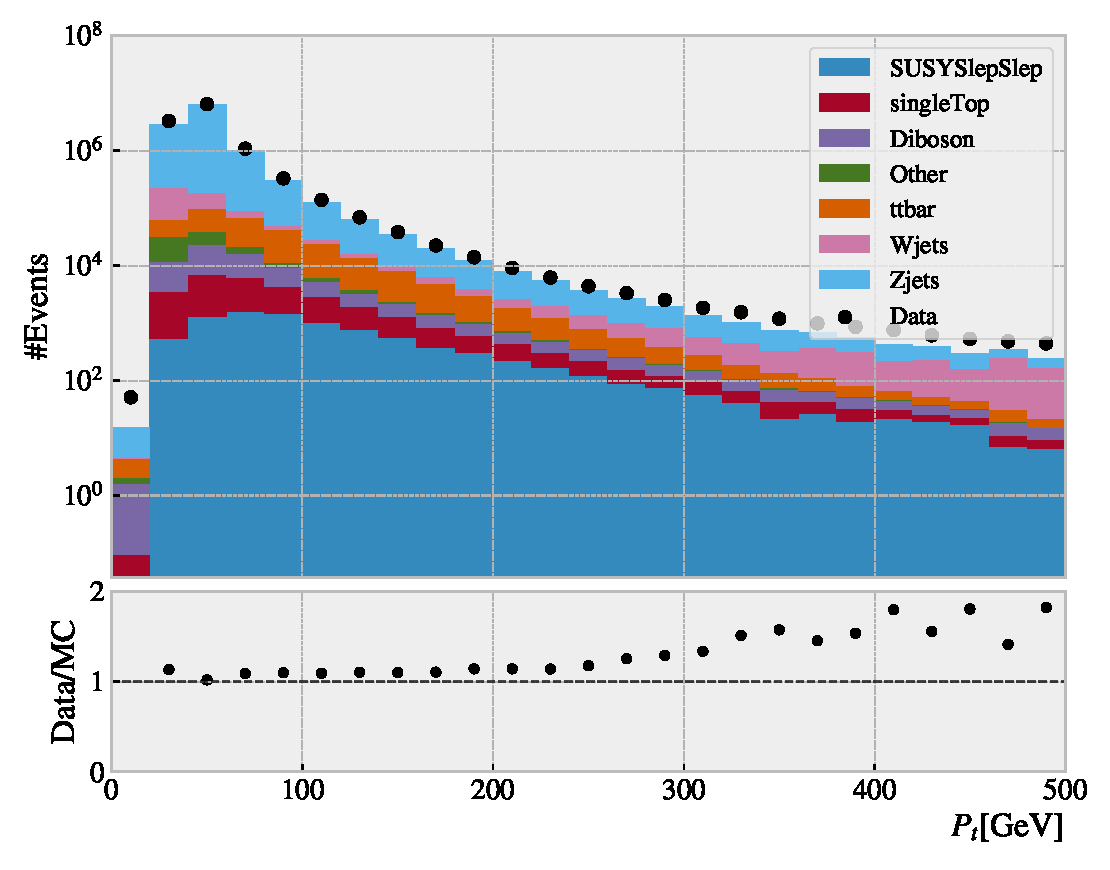
\includegraphics[width=\textwidth]{Figures/Cuts/p_t1.pdf} 
         \caption{}
         \label{fig:Cuts_pt1}
     \end{subfigure}
     \centering
     \begin{subfigure}[b]{.6\textwidth}
         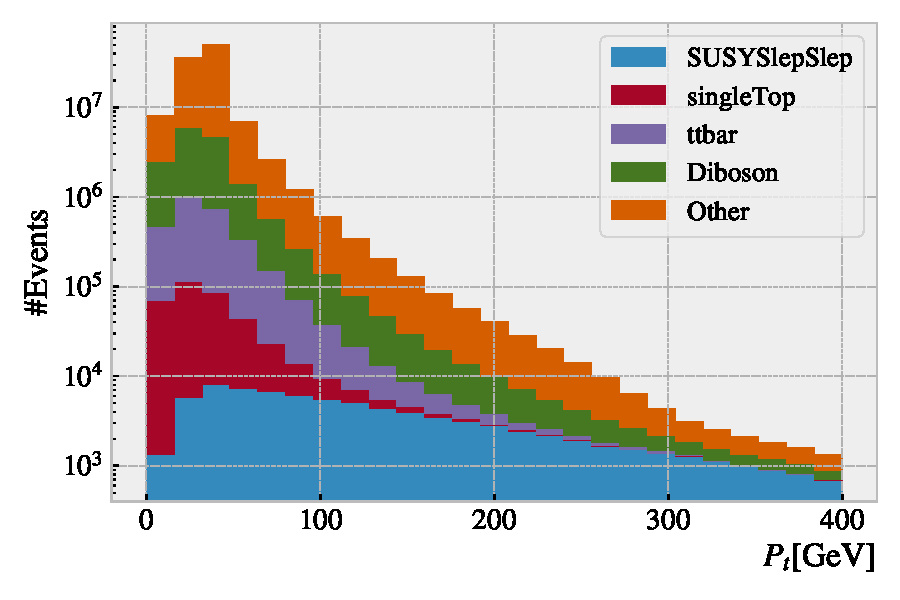
\includegraphics[width=\textwidth]{Figures/Cuts/p_t2.pdf} 
         \caption{}
         \label{fig:Cuts_pt2}
     \end{subfigure}
    }
     \makebox[\linewidth][c]{%
     \centering
     \begin{subfigure}[b]{.6\textwidth}
         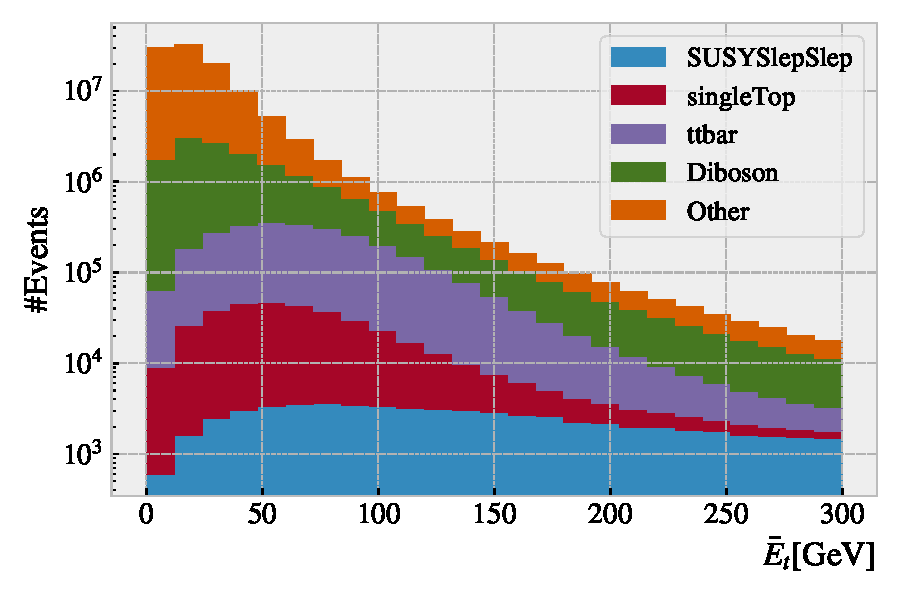
\includegraphics[width=\textwidth]{Figures/Cuts/MET.pdf} 
         \caption{}
         \label{fig:Cuts_met}
     \end{subfigure}
     \centering
     \begin{subfigure}[b]{.6\textwidth}
         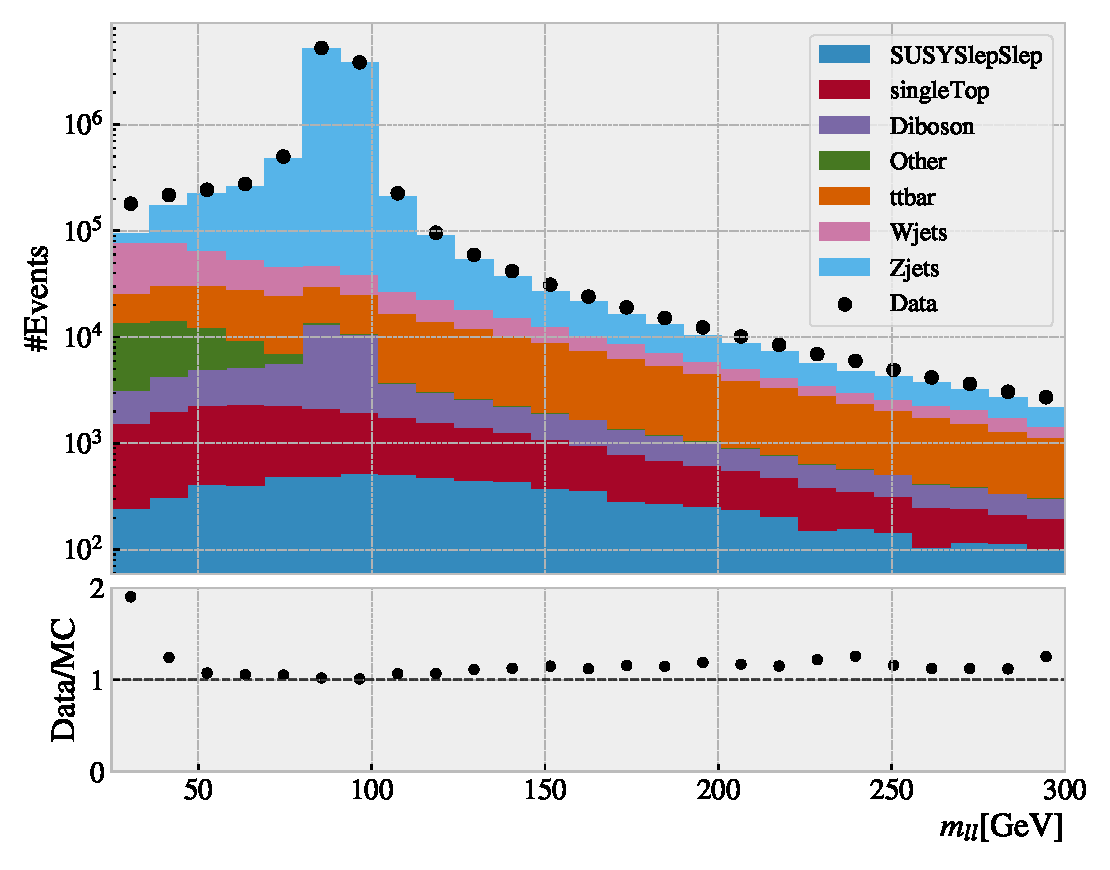
\includegraphics[width=\textwidth]{Figures/Cuts/mll.pdf} 
         \caption{}
         \label{fig:Cuts_mll}
     \end{subfigure}
    }
    \centering
    \begin{subfigure}[b]{.65\textwidth}
         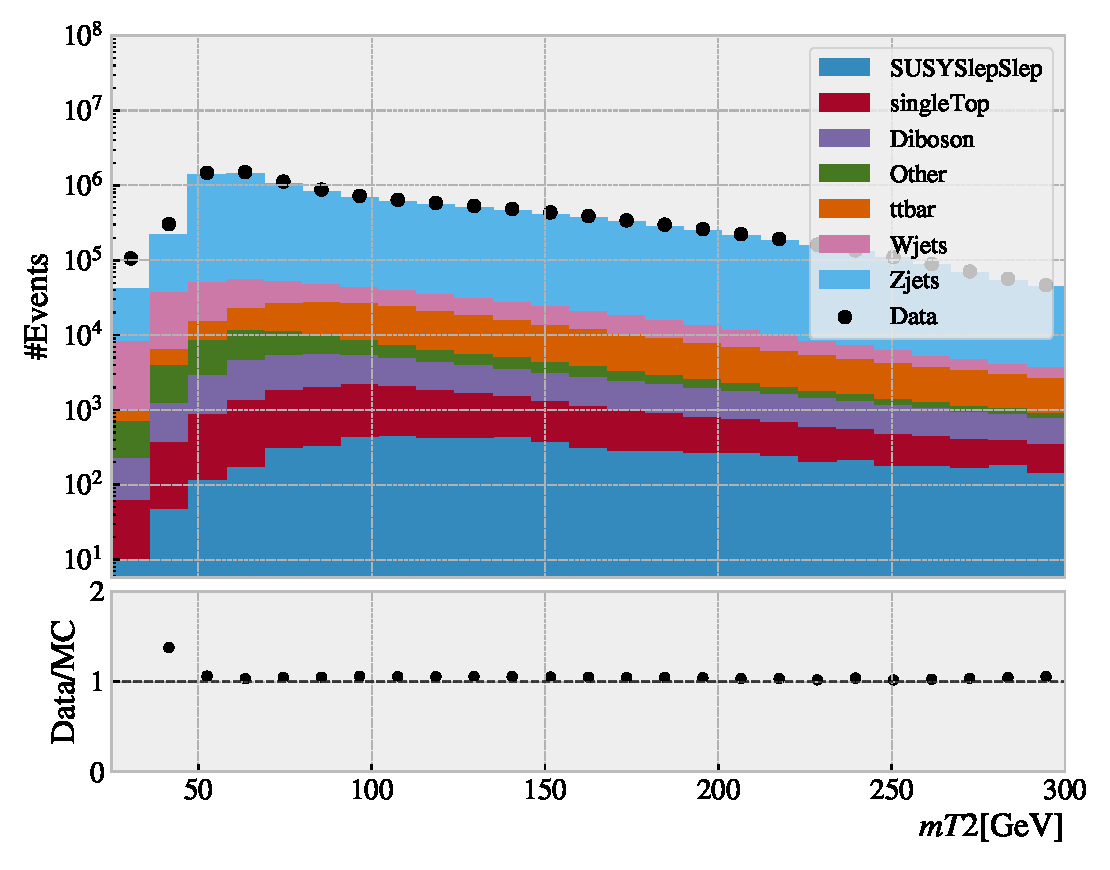
\includegraphics[width=\textwidth]{Figures/Cuts/mT2.pdf}
         \caption{}
         \label{fig:Cuts_T2}
    \end{subfigure}
    \hfill
    \caption{The distribution of transverse momentum of first \ref{fig:Cuts_pt1} and second \ref{fig:Cuts_pt2} lepton, missing transverse energy \ref{fig:Cuts_met}, dilepton mass \ref{fig:Cuts_mll} and the stransverse mass \ref{fig:Cuts_T2} for the MC and real data.
    \label{fig:var1}}
\end{figure}

\begin{figure}
    \makebox[\linewidth][c]{%
     \centering
     \begin{subfigure}[b]{.6\textwidth}
         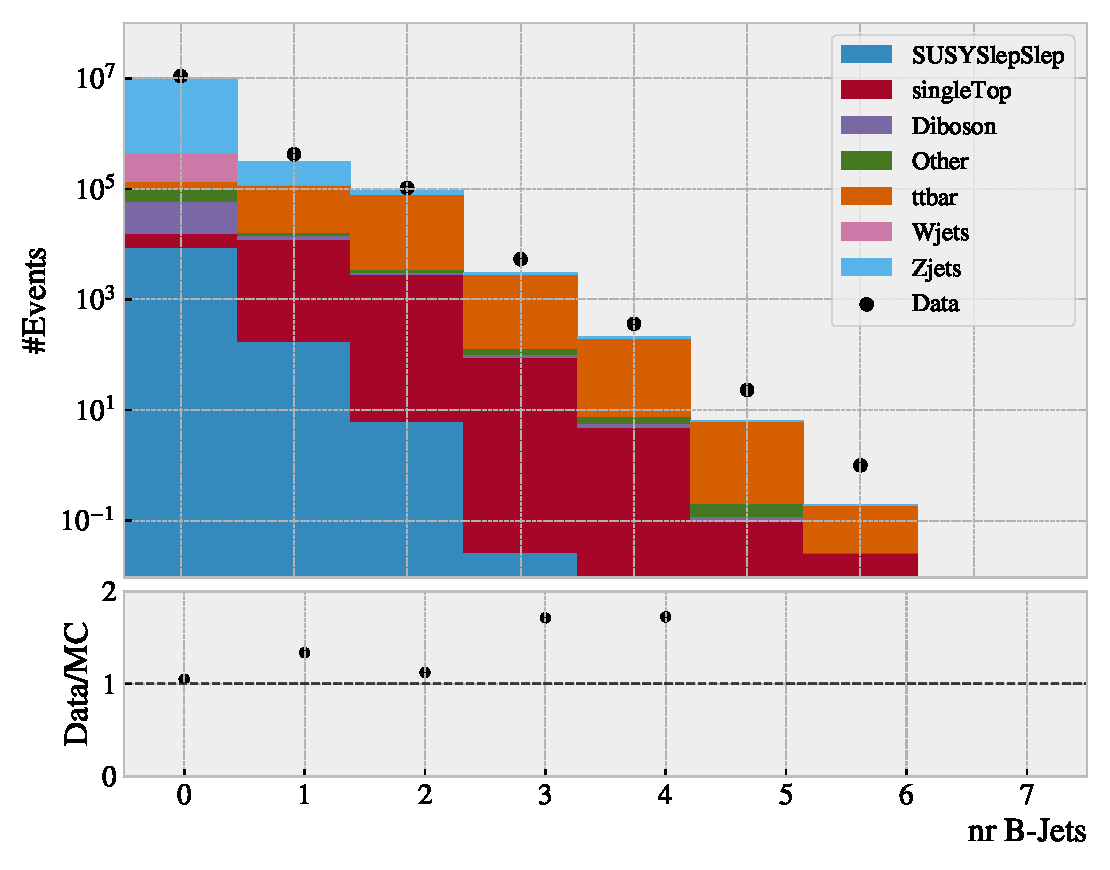
\includegraphics[width=\textwidth]{Figures/Cuts/bTag.pdf} 
         \caption{Nr B-Jets}
         \label{fig:Cuts_bTag}
     \end{subfigure}
     \centering
     \begin{subfigure}[b]{.6\textwidth}
         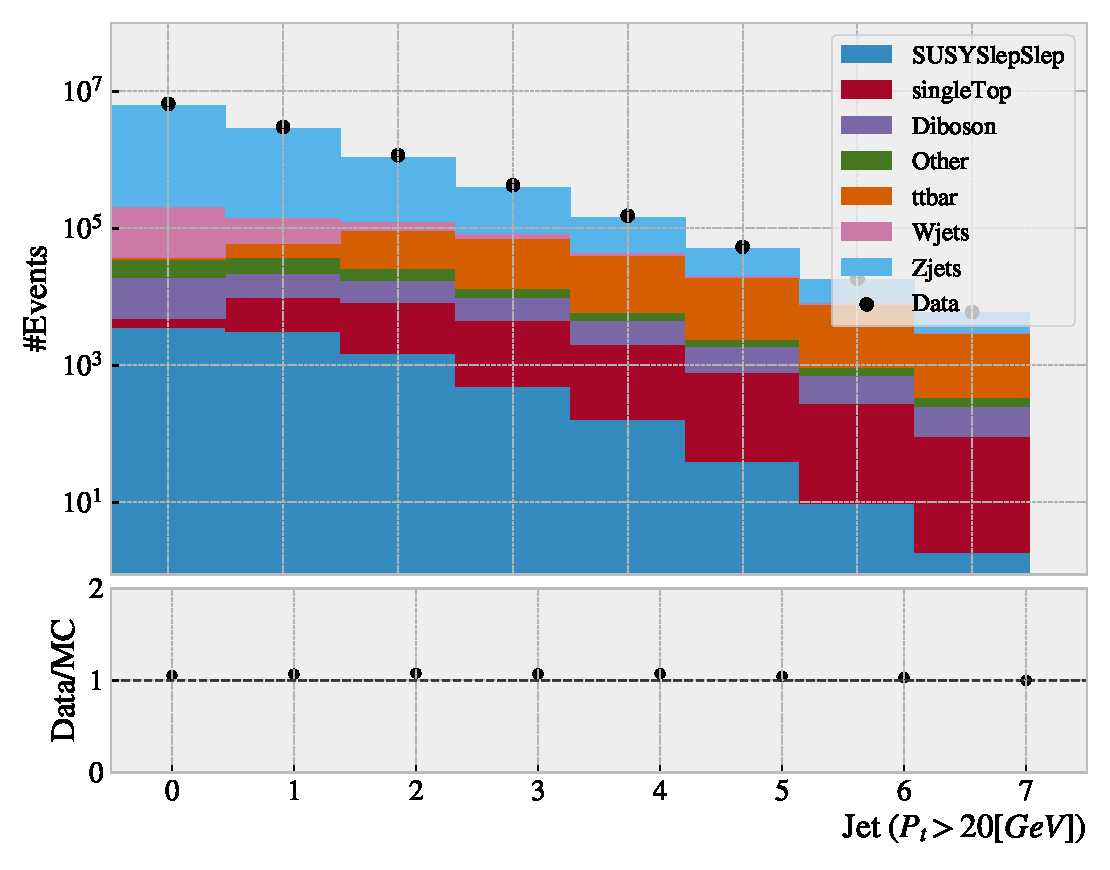
\includegraphics[width=\textwidth]{Figures/Cuts/njet20.pdf} 
         \caption{Jets with a transverse momentum above 20[GeV]}
         \label{fig:Cuts_jet20}
     \end{subfigure}
    }
     \makebox[\linewidth][c]{%
     \centering
     \begin{subfigure}[b]{.6\textwidth}
         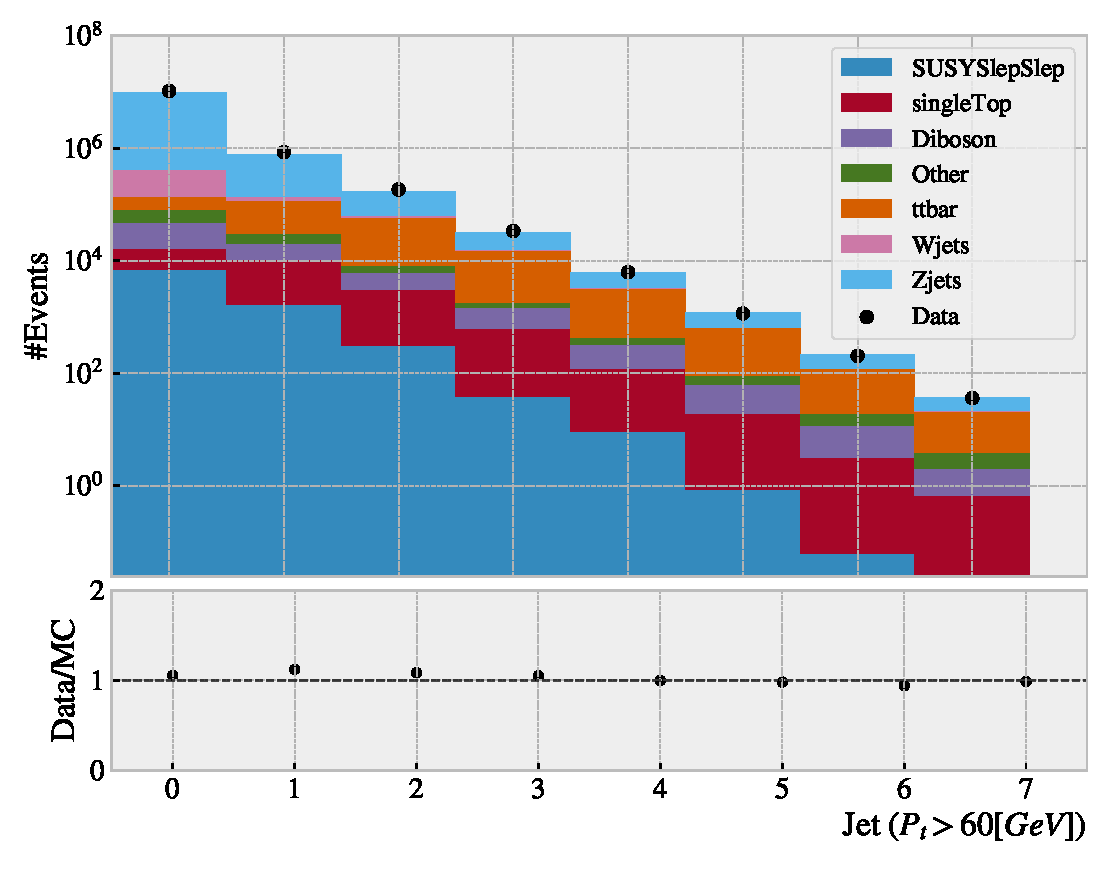
\includegraphics[width=\textwidth]{Figures/Cuts/njet60.pdf} 
         \caption{Jets with a transverse momentum above 60[GeV]}
         \label{fig:Cuts_jet60}
     \end{subfigure}
     \centering
     \begin{subfigure}[b]{.6\textwidth}
         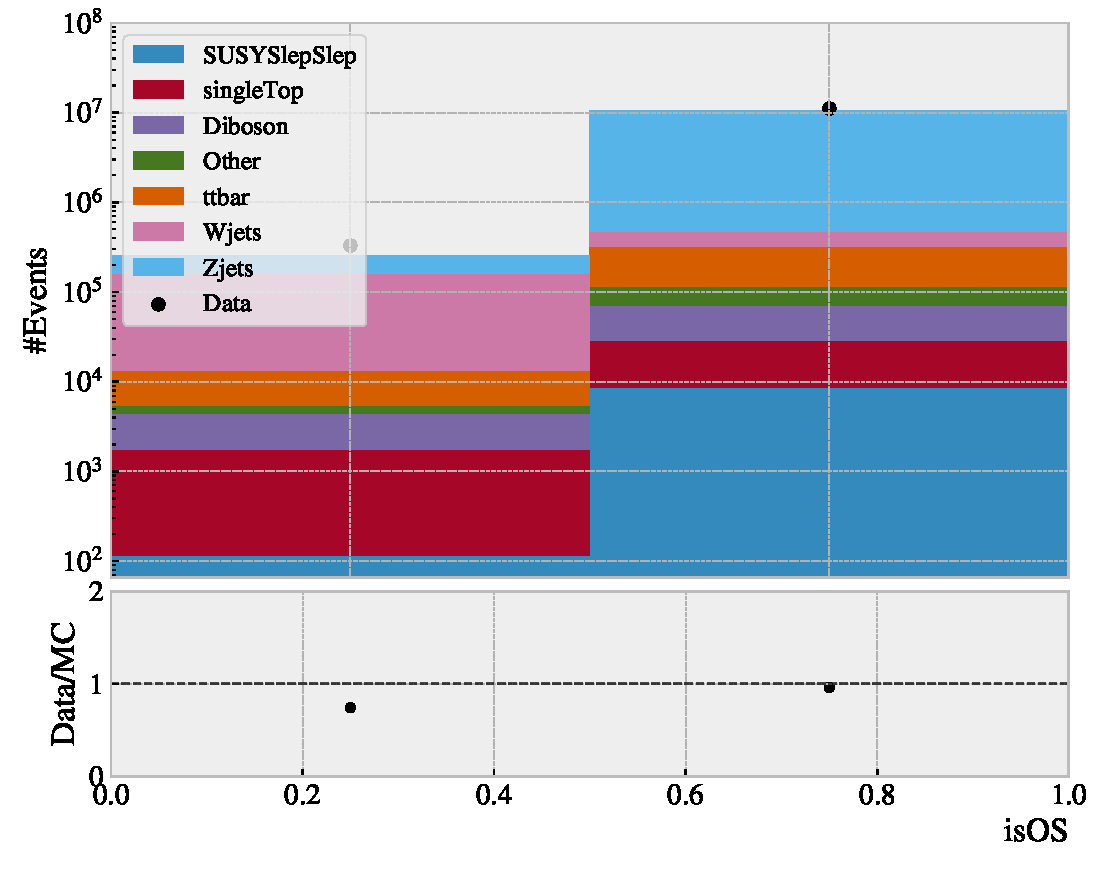
\includegraphics[width=\textwidth]{Figures/Cuts/isOS.pdf} 
         \caption{Is lepton pair opposite charge}
         \label{fig:Cuts_isOS}
     \end{subfigure}
    }
    \caption{}
    \label{fig:var2}
\end{figure}
\subsection{Cuts for AR}
In this section I will present the cuts made to define the AR as well as the result from applying them to the full data set. By studying the distribution plots in figure \ref{fig:var1} and \ref{fig:var1}, I aimed to remove as much of the background by making cuts before any of the peaks for the SUSY signal. By doing so I defined the region as presented by the cuts in table \ref{table:AR}. Note that the cut applied on the missing transverse energy is the only case were a upper-limit is defined. This was done as an attempt to remove regions were the MC and real data differ in a unsystematic way.
\bgroup
\title{TBD}
{\tabcolsep=20pt
\begin{table}
    \caption{Feature cuts in AR}
    \label{table:AR}
    \centering 
    \begin{threeparttable}
    \begin{tabular}{ccc}
    Features & & Thresholds\\
     \midrule\midrule
    $\bar{E}_t$   & &  $> 50, \ < 250[GeV]$  \\%new row
    \cmidrule(l  r ){1-3}
     $P_t \ (1)$ & &  $> 80[GeV]$  \\ 
    \cmidrule(l r ){1-3}
     $P_t \ (2)$ & & $>25[GeV]$  \\ 
    \cmidrule(l r ){1-3}
    $m_{ll}$ & & $>120[GeV]$  \\
    \cmidrule(l r ){1-3}
    $m_{T2}$  & & $>175[GeV]$ \\
    \cmidrule(l r ){1-3}
    $Nr\ B-Jet$ & & $<2$  \\ 
    \cmidrule(l r ){1-3}
    $isOS$ & & $True$  \\ 
    \cmidrule(l r ){1-3}
    $isSS$ & & $False$  \\ 
    \midrule\midrule
    \end{tabular}
    \end{threeparttable}
\end{table}
}
\egroup
\newline
By applying the cuts for the AR a great amount of the data was removed. The resulting reduction on each channel is presented in table \ref{table:AR_result}. From the table we can see that Z+jets and W+jets was effected the most, removing more than $99.99\%$ from both channels. Dibson and ttbar were reduced $96\%$ and $94\%$ respectively. As expected this channels are harder to remove given their similiarity to the signal. The others channels was like the Z/W+jets channel almost completely removed. The SUSY-signal was however only reduced by $74\%$ making it the second largest channel in the AR, only beaten by the W+jets channel.
\bgroup
\title{TBD}
{\tabcolsep=20pt
\begin{table}
    \caption{Events analysis of MC-data in total and in AR}
    \label{table:AR_result}
    \begin{threeparttable}
    \makebox[\linewidth][c]{%
    \begin{tabular}{c c c c}
    \textbf{Channel} & \textbf{Nr Event total} & \textbf{Nr Events AR} & \textbf{Reduction [\%]}\\
     \midrule\midrule
    $Diboson$   & $4.5\times 10^{4}$ & $1.5\times 10^{3}$ &  $96\%$  \\%new row
    \cmidrule(l  r ){1-4}
     $ttbar$ & $2.1\times 10^{5}$ & $1.1\times 10^{4}$ & $94\%$  \\ 
    \cmidrule(l r ){1-4}
    $Z+jets$ & $1.0\times 10^{7}$ & $1.9\times 10^{3}$ & $99\%$   \\ 
    \cmidrule(l r ){1-4}
    
    $W+jets$ & $1.0\times 10^{7}$ & $2.7\times 10^{3}$ & $99\%$  \\ 
    \cmidrule(l r ){1-4}
    
    $Others$  & $3.7\times 10^{5}$ & $6.2\times 10^{1}$ & $99\%$ \\

    \cmidrule(l r ){1-4}

    $SUSYSlepSlep$  &  $8.8\times 10^{3}$ & $2.3\times 10^{3}$ & $74\%$ \\
    \midrule\midrule
    \end{tabular}
    }
    \end{threeparttable}
\end{table}
}
\egroup
\subsection{Training and validation}
As mentioned in section \ref{sec:DH}, all training, validation and testing was done in in the AR. Firstly I preformed a fit of the classifier on the training set, containing $80\%$ of the signal and background. After training I plotted the distribution as well as the ROC-curve of the output from the classifier from the training data. The results are shown in figure \ref{fig:XGB_dist_training} and \ref{fig:XGB_dist_validation} . Figure \ref{fig:XGB_dist_training} shows a clear separation between the background and signal. This is evident from the ROC-curve which creates an area of 0.985. 
\begin{figure}
    \makebox[\linewidth][c]{%
     \centering
     \begin{subfigure}[b]{.6\textwidth}
         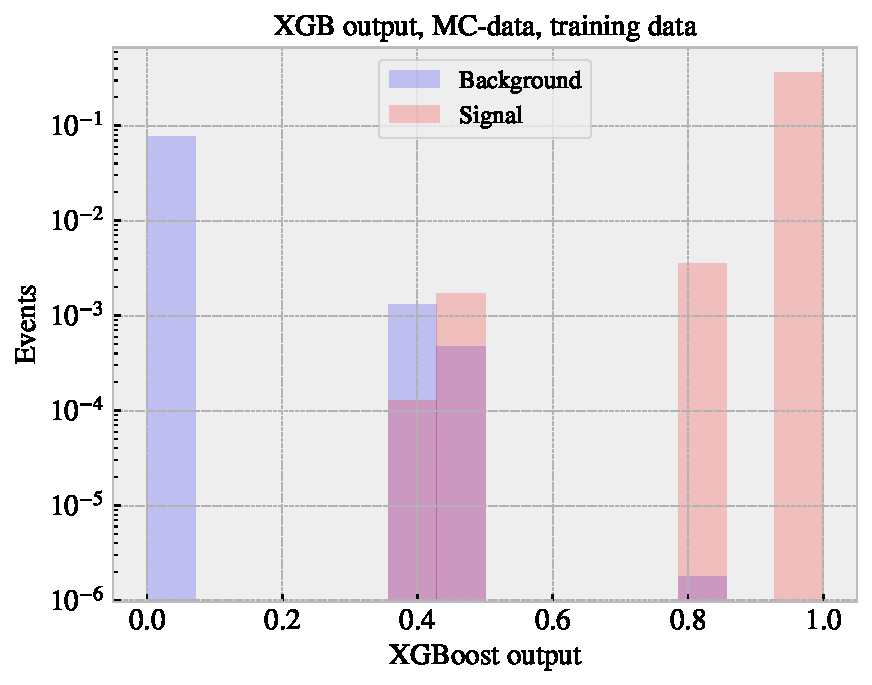
\includegraphics[width=\textwidth]{Figures/Training/train.pdf}
         \caption{}
         \label{fig:XGB_dist_training}
     \end{subfigure}
     \hfill
     \begin{subfigure}[b]{.6\textwidth}
         \includegraphics[width=\textwidth]{Figures/Training/train_ROC.pdf}
         \caption{}
         \label{fig:XGB_ROC_training}
     \end{subfigure}
    }
    \caption{The output distribution \ref{fig:XGB_dist_training} and the ROC-curve \ref{fig:XGB_ROC_training} produced by the XGBoost-classifier on training data. }
\end{figure}
\newline
After training and analysing the reuslts on the training data, I create similar plots for the validation data. The distribution and ROC-curve is displayed in figures \ref{fig:XGB_dist_validation}
and \ref{fig:XGB_ROC_validation}. In figure \ref{fig:XGB_dist_validation} we see a clear separation between the signal and background, although not as prominent as in the training data. From figure \ref{fig:XGB_ROC_validation} we see that the classifier achieves an excellent ROC-curve area of 0.963. It is clear from the validation data that the XGBoost has picked up differences in trend for the signal and background and will be an can be used as a tool in the hope to create a effective signal region. 
\newline
\begin{figure}
    \makebox[\linewidth][c]{%
     \centering
     \begin{subfigure}[b]{.6\textwidth}
         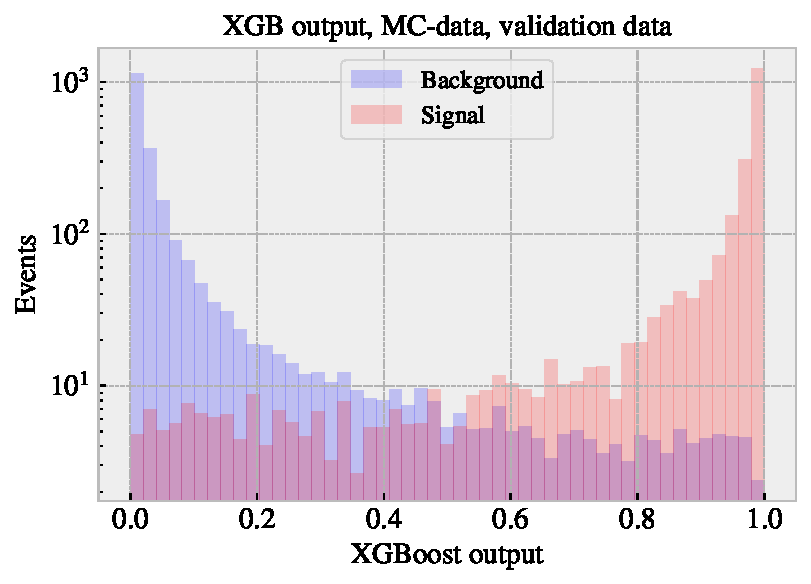
\includegraphics[width=\textwidth]{Figures/Training/validation.pdf}
         \caption{}
         \label{fig:XGB_dist_validation}
     \end{subfigure}
     \hfill
     \begin{subfigure}[b]{.6\textwidth}
         \includegraphics[width=\textwidth]{Figures/Training/validation_ROC.pdf}
         \caption{}
         \label{fig:XGB_ROC_validation}
     \end{subfigure}
    }
    \caption{The output distribution \ref{fig:XGB_dist_validation} and the ROC-curve \ref{fig:XGB_ROC_validation} produced by the XGBoost-classifier on validation data.}
\end{figure}
Finally we plot the distribution of all the background data in figure \ref{fig:XGB_dist_background}. The figure displays the classifiers ability to separate more than $90\%$ of the MC background to the lowest values of the output. 
\begin{figure}
    \centering
    \includegraphics[width=0.8\linewidth]{Figures/Training/BackgroundMC.pdf}
    \caption{The output distribution of the XGBoost on all background MC data.}
    \label{fig:XGB_dist_background}
\end{figure}
\subsection{Cuts for SR1}
\begin{figure}
\bgroup
\title{TBD}
{\tabcolsep=20pt
\begin{table}[H]
    \caption{Events analsysis of MC-data in total and in SR1}
    \centering 
    \begin{threeparttable}
    \makebox[\linewidth][c]{%
    \begin{tabular}{c c c c}
    \textbf{Channel} & \textbf{Nr Event AR} & \textbf{Nr Events SR1} & \textbf{Reduction [\%]}\\
     \midrule\midrule
    $Diboson$   & $1.5\times 10^{3}$ & $3.3\times 10^{2}$ &  $78\%$  \\%new row
    \cmidrule(l  r ){1-4}
     $ttbar$ & $1.1\times 10^{4}$ & $4.4\times 10^{2}$ & $96\%$  \\ 
    \cmidrule(l r ){1-4}
    $Z+jets$ & $1.9\times 10^{3}$ & $3.1\times 10^{2}$ & $83\%$   \\ 
    \cmidrule(l r ){1-4}
    
    $W+jets$ & $2.7\times 10^{3}$ & $4.0\times 10^{1}$ & $99\%$  \\ 
    \cmidrule(l r ){1-4}

    $Others$  & $6.2\times 10^{1}$ & $1.0\times 10^{1}$ & $84\%$ \\
    \cmidrule(l r ){1-4}

    $SUSYSlepSlep$  &  $2.3\times 10^{3}$ & $1.8\times 10^{3}$ & $21\%$ \\
    \midrule\midrule
    \end{tabular}
    }
    \end{threeparttable}
    \label{table:AMS}
\end{table}
}
\egroup
\end{figure}
\subsection{Cuts for SR2}
\begin{figure}
\bgroup
\title{TBD}
{\tabcolsep=20pt
\begin{table}[H]
    \caption{Events analsysis of MC-data in total and in SR2}
    \centering 
    \begin{threeparttable}
    \makebox[\linewidth][c]{%
    \begin{tabular}{c c c c}
    \textbf{Channel} & \textbf{Nr Event AR} & \textbf{Nr Events SR1} & \textbf{Reduction [\%]}\\
     \midrule\midrule
    $Diboson$   & $1.5\times 10^{3}$ & $6\times 10^{1}$ &  $78\%$  \\%new row
    \cmidrule(l  r ){1-4}
     $ttbar$ & $1.1\times 10^{4}$ & $4.5\times 10^{1}$ & $96\%$  \\ 
    \cmidrule(l r ){1-4}
    $Z+jets$ & $1.9\times 10^{3}$ & $5.2\times 10^{2}$ & $83\%$   \\ 
    \cmidrule(l r ){1-4}
    
    $W+jets$ & $2.7\times 10^{3}$ & $4.0\times 10^{1}$ & $99\%$  \\ 
    \cmidrule(l r ){1-4}

    $Others$  & $6.2\times 10^{1}$ & $1.0\times 10^{1}$ & $84\%$ \\
    \cmidrule(l r ){1-4}

    $SUSYSlepSlep$  &  $2.3\times 10^{3}$ & $1.8\times 10^{3}$ & $21\%$ \\
    \midrule\midrule
    \end{tabular}
    }
    \end{threeparttable}
    \label{table:AMS}
\end{table}
}
\egroup
\end{figure}
\subsection{Results in SR1 and SR2}
\bgroup
\centering
\title{TBD}
{\tabcolsep=20pt
\begin{table}[H]
    \centering
    \caption{Exclusion of slepton and neutralino massses.}
    \centering 
    \begin{threeparttable}
    \makebox[\linewidth][c]{%
    \begin{tabular}{ccc}
    \textbf{Masses[GeV]} &  \textbf{Events in SR1 [efficiency]} & \textbf{Events in SR2 [efficiency]}  \\
     \midrule\midrule
    $m_{\tilde{l}} = 100$, $m_{\tilde{\chi}} = 50$   & 736  & $Y$   \\%new row
    \cmidrule(l  r ){1-3}
     $m_{\tilde{l}} = 100.5$, $m_{\tilde{\chi}}  = 1$ & 1309 &  $Y$  \\ 
    \cmidrule(l r ){1-3}
    $m_{\tilde{l}} = 200$, $m_{\tilde{\chi}}  = 100$ & 199 & $Y$  \\ 
    \cmidrule(l r ){1-3}

    $m_{\tilde{l}} = 200.5$, $m_{\tilde{\chi}} = 1$  & 278 & $Y$   \\% end of rows
    \cmidrule(l r ){1-3}
    
    $m_{\tilde{l}} = 300$, $m_{\tilde{\chi}}  = 200$  & 43 &   $N$ \\
    \cmidrule(l r ){1-3}
    
    $m_{\tilde{l}} = 300.5$, $m_{\tilde{\chi}}  = 1$  & 64  &   $N$ \\
    \cmidrule(l r ){1-3}
    
    $m_{\tilde{l}} = 400$, $m_{\tilde{\chi}}  = 300$  & 12  &   $N$ \\
    \cmidrule(l r ){1-3}
    
    $m_{\tilde{l}} = 500$, $m_{\tilde{\chi}}  = 100$  & 6 &   $N$ \\
    \cmidrule(l r ){1-3}
    
    $m_{\tilde{l}} = 500$, $m_{\tilde{\chi}}  = 100$  &  7 &   $N$ \\
    \cmidrule(l r ){1-3}
    
    $m_{\tilde{l}} = 500.5$, $m_{\tilde{\chi}}  = 1$  & 7  &   $N$ \\
    \cmidrule(l r ){1-3}
    
    $m_{\tilde{l}} = 600$, $m_{\tilde{\chi}}  = 1$  & 3  &   $N$ \\
    \cmidrule(l r ){1-3}
    
    $m_{\tilde{l}} = 600$, $m_{\tilde{\chi}}  = 300$  & 3 &   $N$ \\
    \cmidrule(l r ){1-3}
    
    $m_{\tilde{l}} =  700$, $m_{\tilde{\chi}}  = 300$  & 1  &   $N$ \\
    \cmidrule(l r ){1-3}
    
    $m_{\tilde{l}} =  700.5$, $m_{\tilde{\chi}}  = 1$  &  1
    &   $N$ \\
    \midrule\midrule
    \end{tabular}
    }
    \end{threeparttable}
    \label{table:AMS}
\end{table}
}
\egroup
\begin{figure}
    \makebox[\linewidth][c]{%
     \centering
     \begin{subfigure}[b]{.6\textwidth}
         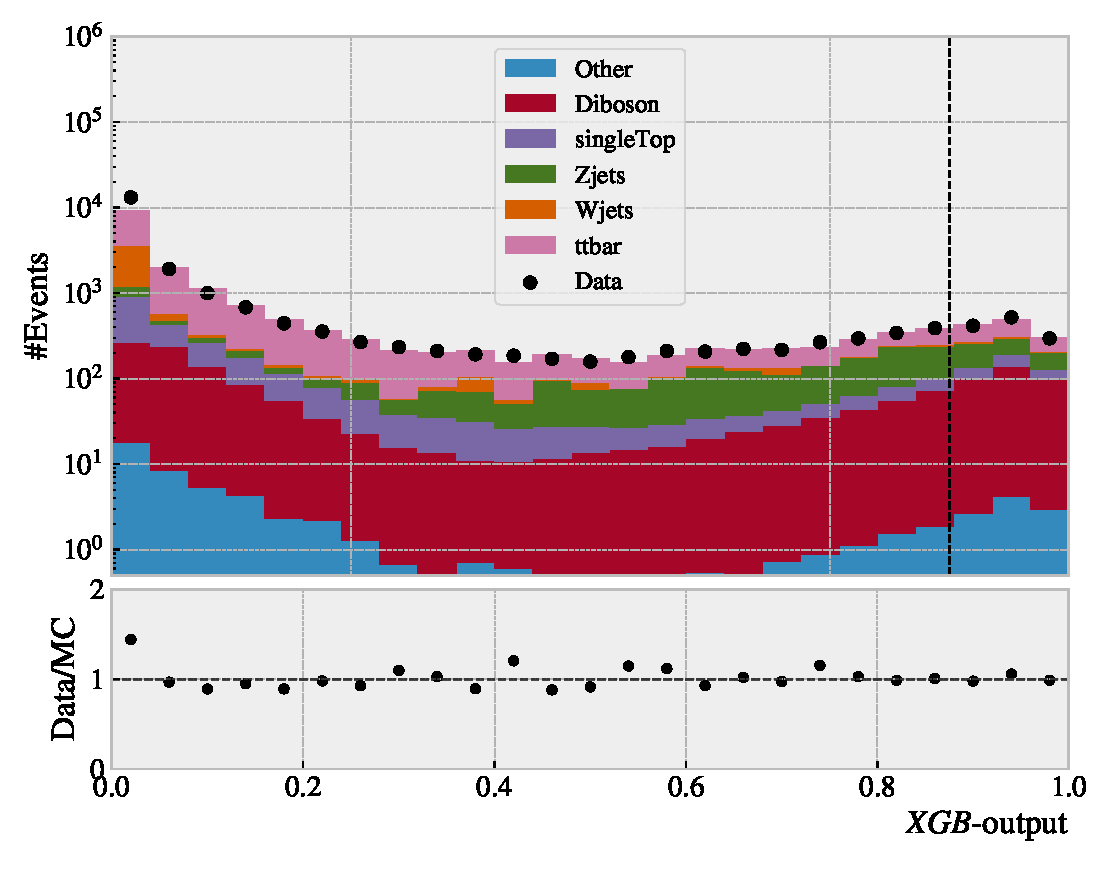
\includegraphics[width=\textwidth]{Figures/Results/XGB_dist.pdf}
         \caption{}
         \label{fig:XGB_SR1}
     \end{subfigure}
     \centering
     \begin{subfigure}[b]{.65\textwidth}
         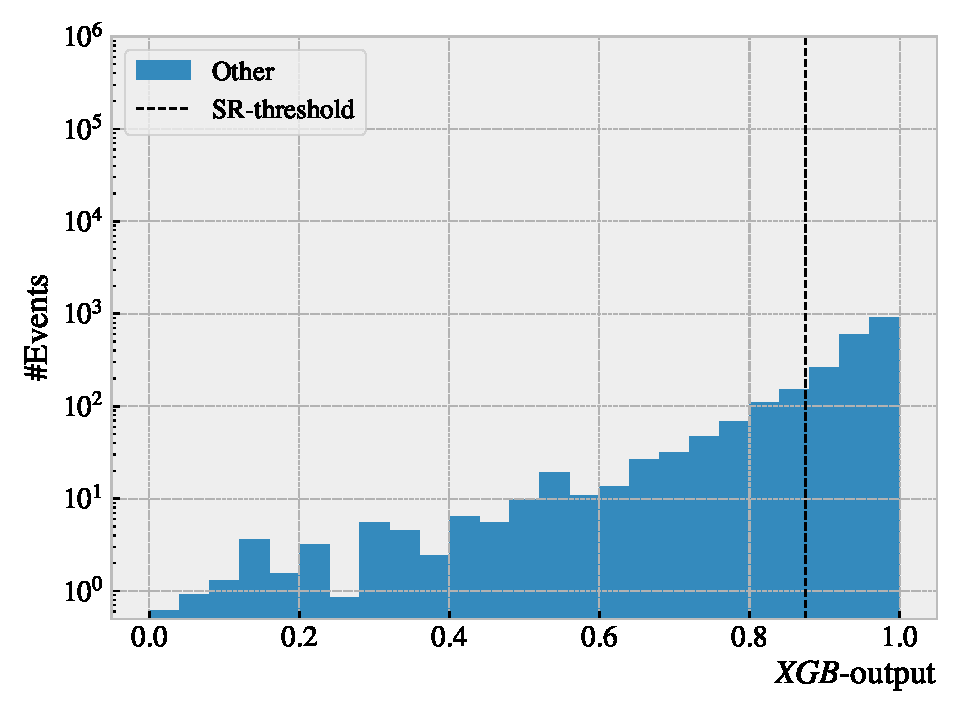
\includegraphics[width=\textwidth]{Figures/Results/XGB_SUSY.pdf}
         \caption{}
         \label{fig:XGB_SUSY}
     \end{subfigure}
    }
    \caption{XGBoost output distribution for MC and data \ref{fig:XGB_SR1} and the SUSYSlepSlep-MC \ref{fig:XGB_SUSY} in SR1.}
\end{figure}
\begin{figure}
    \makebox[\linewidth][c]{%
     \centering
     \begin{subfigure}[b]{\textwidth}
         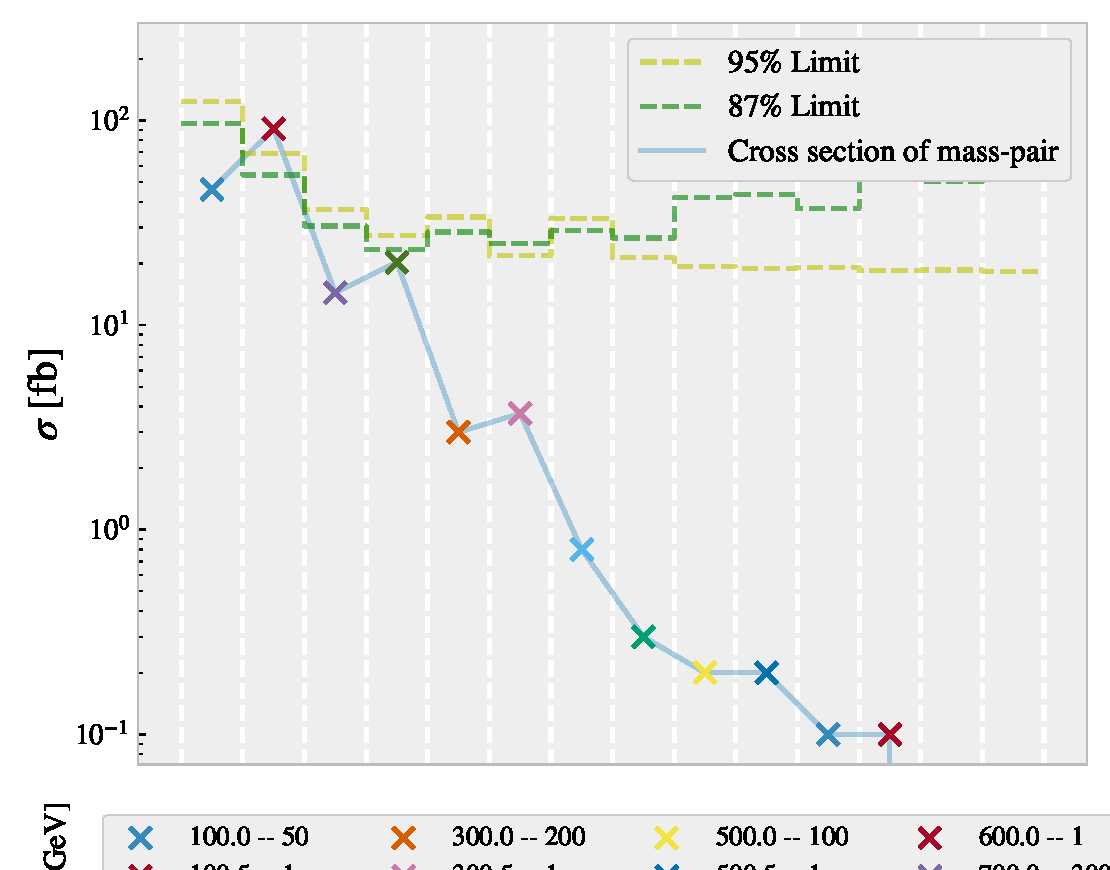
\includegraphics[width=\textwidth]{Figures/Results/ExlusionEvents.pdf}
     \end{subfigure}
     }
     \caption{Visualization of crossection of each mass-pair in SR2 with each corresponding exclusion limit up to $95\%$ and $87\%$.}
     \label{fig:ExlusionSR2}
\end{figure}
\begin{figure}
    \makebox[\linewidth][c]{%
     \centering
     \begin{subfigure}[b]{\textwidth}
         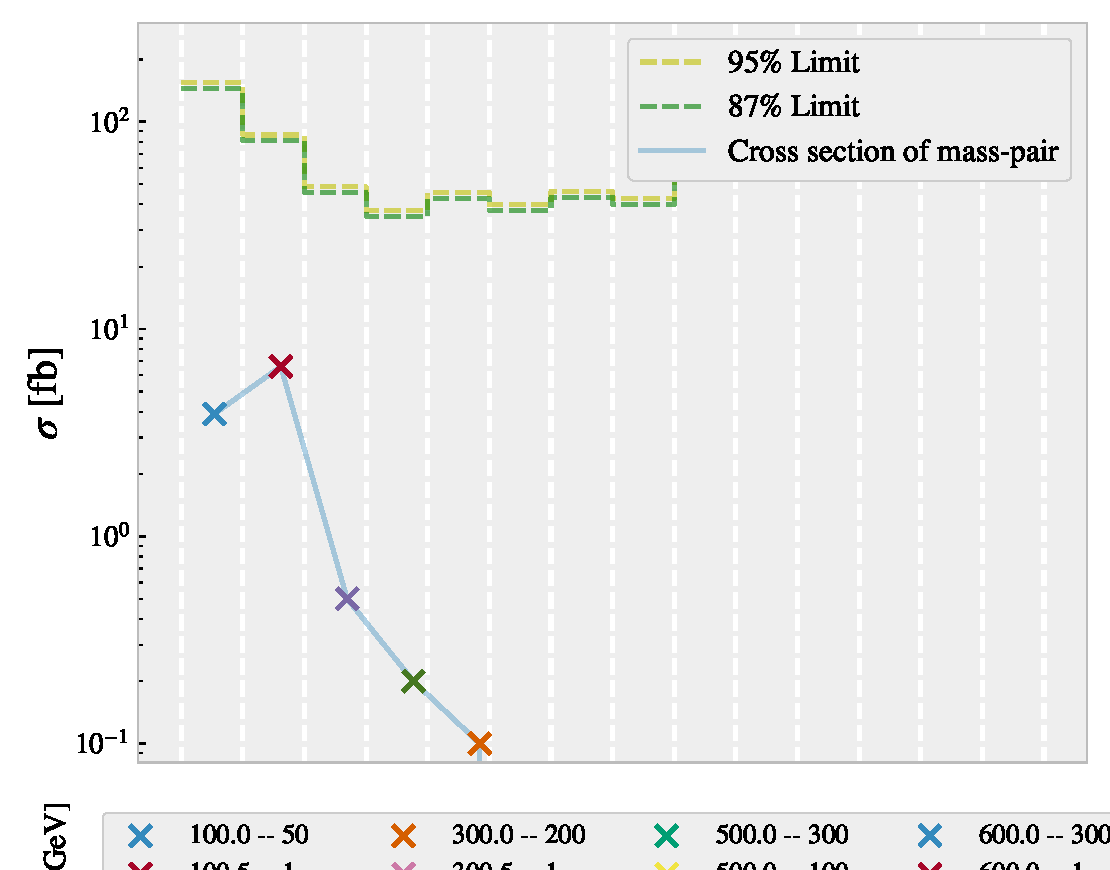
\includegraphics[width=\textwidth]{Figures/Results/ExlusionEvents_nML.pdf}
         \caption{Visualization of crossection of each mass-pair in SR3 with each corresponding exclusion limit up to $95\%$ and $87\%$.}
         \label{fig:ExlusionSR3}
     \end{subfigure}
    }
\end{figure}


\subsection{The way forward}
\begin{itemize}
    \item More data
    \item Individual SR for each mass. Some masses prefer a stricter threshold on ML
    \item New way of handling negative weights. Cell resampling (https://arxiv.org/pdf/2109.07851.pdf)
    \item More data on Jets, possibly exclude more Z+Jets and W+Jets before ML-Cut
\end{itemize}

\section{Conclusion}
\newpage
\printbibliography

\end{document}
